\documentclass{standalone}
\usepackage{xcolor}
\usepackage{verbatim}
\usepackage[T1]{fontenc}
\usepackage{graphics}
\usepackage{hyperref}
\newcommand{\code}[1]{\texttt{#1}}
\newcommand{\R}{R}
\newcommand{\pkg}[1]{#1}
\newcommand{\CRANpkg}[1]{\pkg{#1}}%
\newcommand{\BIOpkg}[1]{\pkg{#1}}
\usepackage{amsmath,amssymb,array}
\usepackage{booktabs}
\usepackage{lscape}
\usepackage{bm}
\usepackage{mathrsfs}
\usepackage{graphicx}
\usepackage{tablefootnote}
\usepackage{footmisc}
\usepackage{pdflscape}
\usepackage{enumerate}
\usepackage[shortlabels]{enumitem}
\usepackage{afterpage}
\usepackage{makecell}
\usepackage{capt-of}% or use the larger `caption` package
\usepackage{subfig}
\usepackage{listings}
\usepackage{adjustbox}
\usepackage{multirow}
\usepackage{booktabs}
\usepackage{tikz}
\usetikzlibrary{matrix,calc,shapes,arrows}
\usetikzlibrary{shapes.multipart} 
\tikzset{
  treenode/.style = {shape=rectangle, rounded corners,
                     draw,align=center,
                     top color=white,
                     text width = 4.1cm,
                     inner sep=2ex,
                     anchor=center},
  treenodel/.style = {shape=rectangle, rounded corners,
                     draw,align=center,
                     top color=white,
                     text width = 2.2cm,
                     inner sep=2ex,
                     anchor=center},
  input/.style = {align=center, text width=4.5cm},
  decision/.style = {treenode, diamond, inner sep=2pt,
                    text width=2cm},
   decisionx/.style = {treenode, diamond, inner sep=2pt,
                    text width=1.5cm},
  decisiond/.style = {treenode, diamond, dashed, inner sep=3pt,
                    text width=2cm},
  treeuc/.style = {treenode,draw=blue,thick},
  treec/.style = {treenode,draw=red,thick},
  treeg/.style = {treenode,draw=green!60,thick,fill=green!5},
  action/.style = {treenode, circle, inner sep=1pt,
                     text width = 3cm},
  root/.style     = {treenode},
  env/.style      = {treenode},
  ginish/.style   = {root},
  dummy/.style    = {circle,draw},
  ar/.style={->,>=latex}
}
\tikzset{connect/.style={rounded corners=#1,
        to path= ($(\tikztostart)!-#1!(\tikztotarget)!-#1!-90:(\tikztotarget)$) -- ($(\tikztotarget)!-#1!(\tikztostart)!-#1!90:(\tikztostart)$) --
        ($(\tikztotarget)!-#1!(\tikztostart)!#1!90:(\tikztostart)$) -- ($(\tikztostart)!-#1!(\tikztotarget)!-#1!90:(\tikztotarget)$) -- cycle (\tikztotarget)
}}
\tikzset{connect/.default=4mm}
\begin{document}
\nopagecolor
\centering
\hspace*{-2cm}
\resizebox{1000em}{!}{%
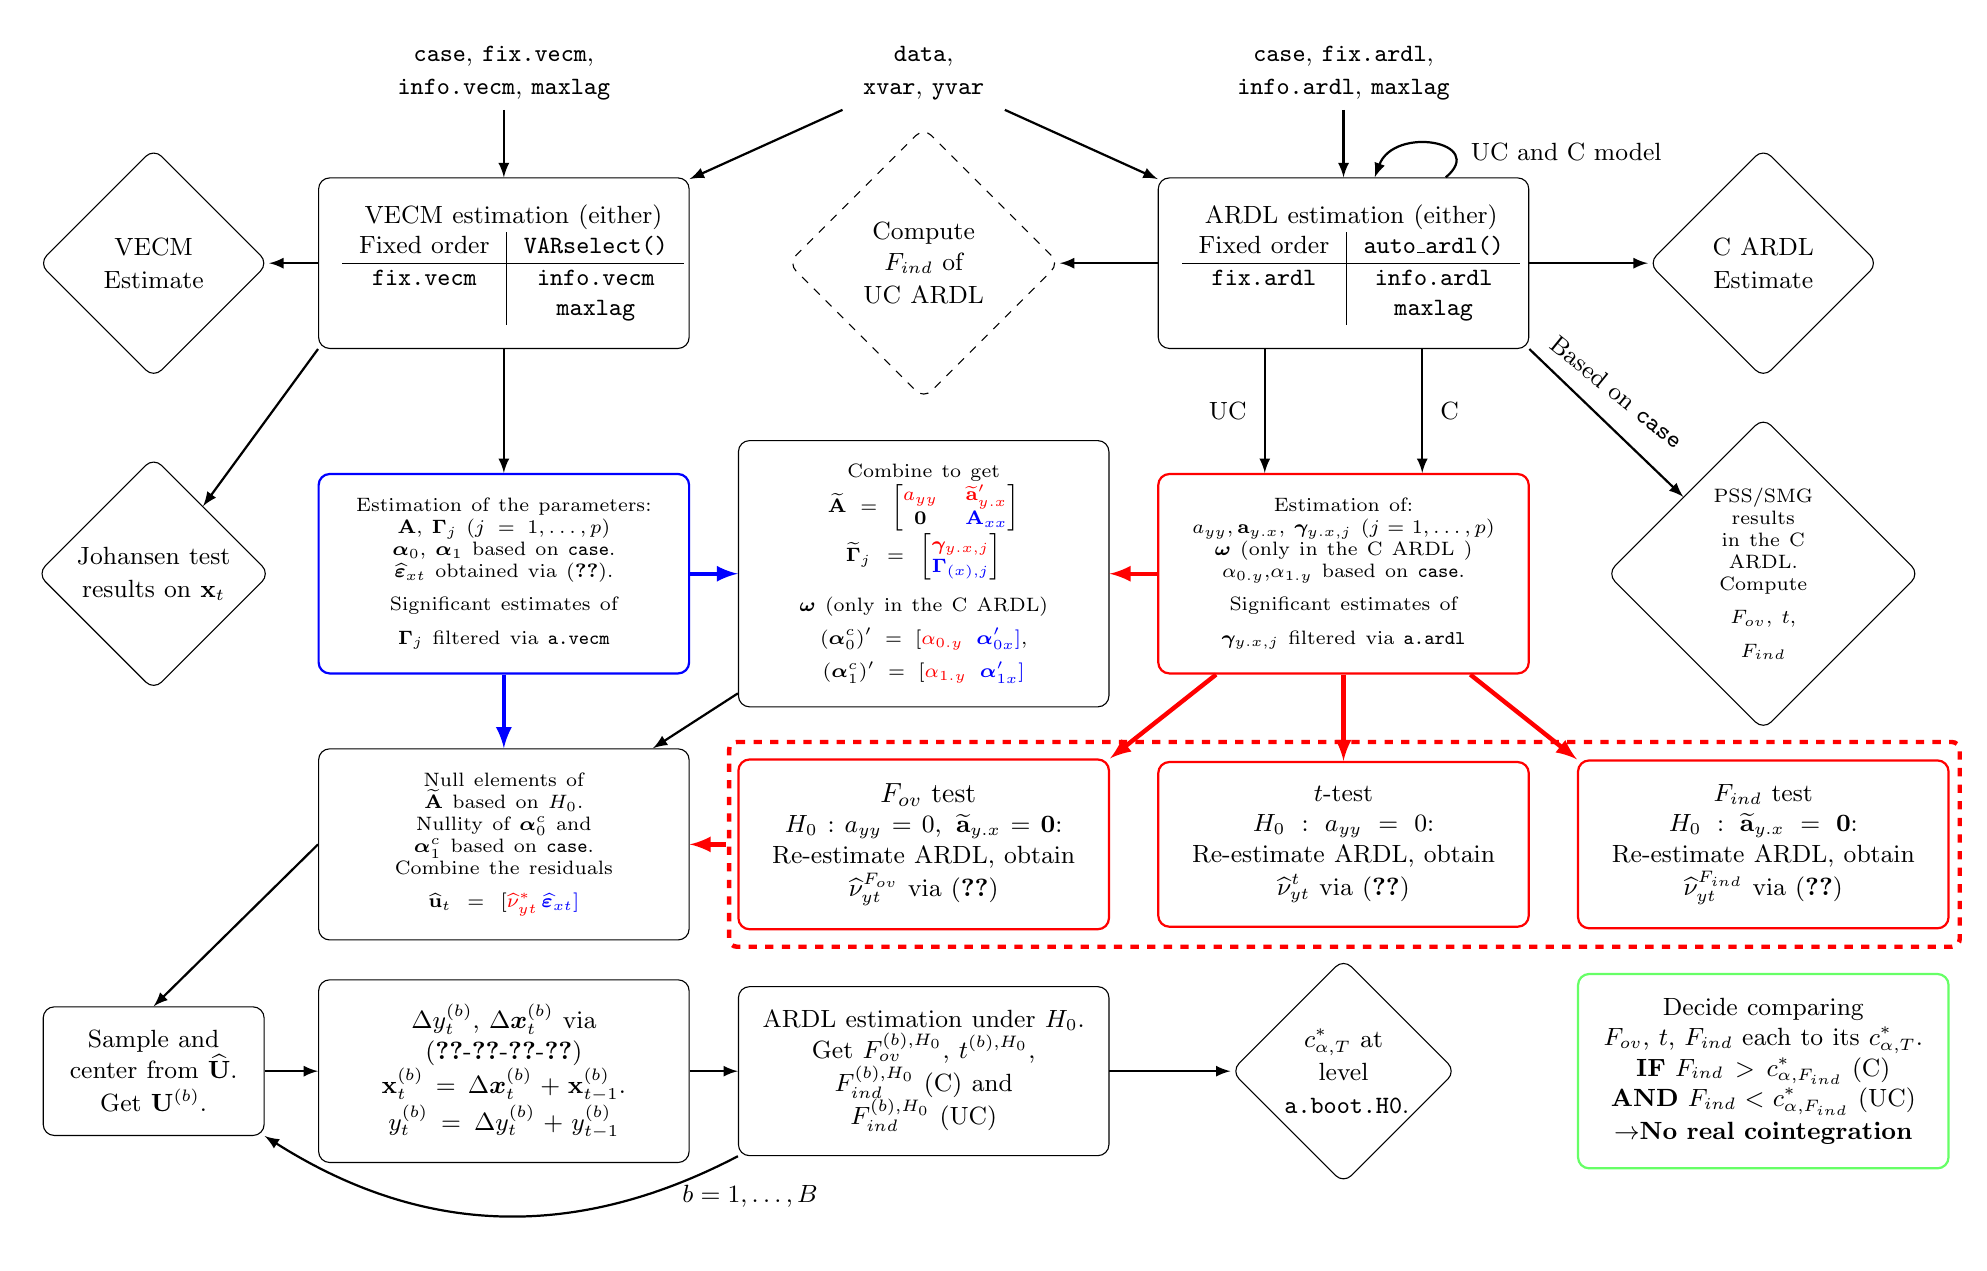
\begin{tikzpicture}[-latex][scale=0.3]
  \matrix (chart)[ampersand replacement=\#]
    [
      matrix of nodes,
      column sep      = 1.7em,
      row sep         = 1.5ex,
      row 2/.style = {nodes={decision}},
      row 5/.style = {nodes={env}}
    ]
    {  %first row
       \#
       |[input]| {\small \texttt{case}, \texttt{fix.vecm},\\
       \texttt{info.vecm}, \texttt{maxlag}}\#
       |[input]| {\small \texttt{data},\\
       \texttt{xvar}, \texttt{yvar}}\#
       |[input]|{\small{\texttt{case}, \texttt{fix.ardl},\\
       \texttt{info.ardl}, \texttt{maxlag}}}
       \#
       \\
       %second row
       |[decision]|{\small
       VECM\\Estimate}
       \normalsize\#
       |[treenode]| {\small
       \centering
       \begin{tabular}{c|c}
       \multicolumn{2}{c}{VECM estimation (either)}\\
        Fixed order & \texttt{VARselect()}\\\hline
        \texttt{fix.vecm} & \texttt{info.vecm}    \\
        &\texttt{maxlag}\\
       \end{tabular}}
       \normalsize\#
       |[decisiond]|{\small
       Compute $F_{ind}$ of \\UC ARDL
       \normalsize}
       \#
       |[treenode]| {\small
       \begin{tabular}{c|c}
       \multicolumn{2}{c}{ARDL estimation (either)}\\
        Fixed order & \texttt{auto\_ardl()}\\\hline
        \texttt{fix.ardl} & \texttt{info.ardl}\\
        &\texttt{maxlag}\\
       \end{tabular}}
       \#
       |[decision]|{\small
       C ARDL\\Estimate}
       \normalsize
       \\
       %third row
       |[decision]|{\small
       Johansen test\\
       results on $\mathbf x_t$}
       \normalsize\#
       |[treeuc]| {\scriptsize
       Estimation of the parameters:\\
       $\mathbf A$, $\boldsymbol\Gamma_j$ $(j=1,\dots,p)$\\
       $\boldsymbol\alpha_0$, $\boldsymbol\alpha_1$  based on \texttt{case}. \\       $\widehat{\boldsymbol\varepsilon}_{xt}$ obtained via \eqref{eq:resvecm}.\\
       Significant estimates of $\boldsymbol\Gamma_j$ filtered via \texttt{a.vecm}}
       \normalsize\#
       |[treenode]|{\scriptsize
        Combine to get \\
        $\widetilde{\mathbf A} =
       \begin{bmatrix}
       \color{red}{a_{yy}} & \color{red} \widetilde{\mathbf{a}}'_{y.x}\\
       {\mathbf 0} & \color{blue}{\mathbf{A}}_{xx}  
       \end{bmatrix}$\\
       $\widetilde{\boldsymbol\Gamma}_j =\begin{bmatrix}\color{red}\boldsymbol{\gamma}_{y.x,j}\\
       \color{blue}\boldsymbol\Gamma_{(x),j}
       \end{bmatrix}$\\
       \phantom{\tiny x}\\
       $\boldsymbol{\omega}$ (only in the C ARDL)\\
       $(\boldsymbol\alpha_{0}^{c})' = [\color{red}{\alpha_{0.y}}\;\color{blue}{\boldsymbol\alpha_{0x}'}]$, $(\boldsymbol\alpha_{1}^{c})' = [\color{red}{\alpha_{1.y}}\;\color{blue}{\boldsymbol\alpha_{1x}'}]$
       \normalsize}
       \#
       |[treec]| {\scriptsize
       Estimation of:\\
       $ a_{yy}, \mathbf{a}_{y.x}$, $\boldsymbol\gamma_{y.x,j}$ $(j=1,\dots,p)$\\
       $\boldsymbol\omega$ (only in the C ARDL )\\
              $\alpha_{0.y}$,$\alpha_{1.y}$ based on \texttt{case}.\\
       Significant estimates of $\boldsymbol\gamma_{y.x,j}$ filtered via \texttt{a.ardl}}
       \normalsize
       \#
       |[decisionx]|{\scriptsize
        PSS/SMG results
        in the C ARDL.
       Compute\\ $F_{ov}$, $t$, $F_{ind}$}
       \normalsize
       \\
       \#
       |[treenode]|{\scriptsize
       Null elements of $\widetilde{\mathbf A}$ based on $H_0$.\\
       Nullity of $\boldsymbol\alpha_0^c$ and $\boldsymbol\alpha_1^c$ based on \texttt{case}.\\
       Combine the residuals \\
       $\widehat{\mathbf u}_t = [\color{red}\widehat{\nu}_{yt}^{*}\,\color{blue}\widehat{\boldsymbol\varepsilon}_{xt}]$}
       \#
       |[treec]|
       { $F_{ov}$ test \\
       \small$H_0: a_{yy}=0,\; \widetilde{\mathbf{a}}_{y.x}=\mathbf 0$:\\
       Re-estimate ARDL, obtain\\
       $\widehat{\nu}_{yt}^{F_{ov}}$ via \eqref{eq:resfov}
       \normalsize}
       \#
       |[treec]|{\small $t$-test \\$H_0: a_{yy}=0$:\\
       Re-estimate ARDL, obtain\\
       $\widehat{\nu}_{yt}^{t}$ via \eqref{eq:rest}
       \normalsize}
       \#
       |[treec]|{\small $F_{ind}$ test \\$H_0: \widetilde{\mathbf{a}}_{y.x}=\mathbf 0$:\\
       Re-estimate ARDL, obtain\\
       $\widehat{\nu}_{yt}^{F_{ind}}$ via \eqref{eq:resfind}
       \normalsize}
       \\
       |[treenodel]| {\small Sample and \\center
       from $\widehat{\mathbf U}$.\\
       Get ${\mathbf U^{(b)}}$.
       \normalsize}
       \#
       |[treenode]|{\small $\Delta y_t^{(b)}$, $\Delta\boldsymbol x_t^{(b)}$  via (\ref{eq:resfov}-\ref{eq:rest}-\ref{eq:resfind}-\ref{eq:resvecm})\\
       $\mathbf{x}_t^{(b)}=\Delta\boldsymbol x_t^{(b)} + \mathbf{x}_{t-1}^{(b)}$.
       \\
       ${y}_t^{(b)}=\Delta y_t^{(b)} +y_{t-1}^{(b)}$}
       \#
       |[treenode]|{\small ARDL estimation under $H_0$.\\
       Get $F_{ov}^{(b),H_0}$, $t^{(b),H_0}$,\\ $F_{ind}^{(b),H_0}$ (C) and $F_{ind}^{(b),H_0}$ (UC)}
       \#
       |[decisionx]|{\small $c_{\alpha,T}^*$ at level \texttt{a.boot.H0}.}
       \#
       |[treeg]|{\small Decide comparing \\ $F_{ov}$, $t$, $F_{ind}$ each to its $c_{\alpha,T}^{*}$.\\
       \textbf{IF} $F_{ind}>c_{\alpha,F_{ind}}^{*}$ (C)\\
       \textbf{AND} $F_{ind}<c_{\alpha,F_{ind}}^{*}$ (UC)\\
       $\rightarrow$\textbf{No real cointegration}}
       \\
       };
       \draw[thick]
		 (chart-1-3) ->  (chart-2-2);
       \draw[thick]
		 (chart-1-3) -> (chart-2-4);
       \draw[thick]
		 (chart-1-2) -> (chart-2-2);
       \draw[thick]
		 (chart-1-4) -> (chart-2-4);
       \draw[thick]
		 (chart-2-2) -> (chart-2-1);
       \draw[thick]
		 (chart-2-4) -> (chart-2-5);
       \draw[thick]
		 (chart-2-2.south west) -> (chart-3-1);
       \draw[thick]
		 (chart-2-2) -> (chart-3-2);
       \draw[thick]
		 (chart-2-4.south east) to node[right=0.4cm,pos=-0.1,rotate=-39]{\small Based on \texttt{case}} (chart-3-5);
       \draw[ar,thick]
		 ([xshift=-1 cm]chart-2-4.south) to node[left=0.1cm] {\small UC} ([xshift=-1 cm] chart-3-4.north);
       \draw[ar,thick]   ([xshift=1 cm]chart-2-4.south) to node[right=0.1cm] {\small C} ([xshift=1cm] chart-3-4.north);
   \draw[thick] (chart-2-4) edge [in=70, out=40,looseness=2,left=2cm] node[pos=0.3,right=0.1cm]{\small UC and C model\normalsize} (chart-2-4);
   \draw[thick]
		 (chart-2-4) -> (chart-2-3);
   \draw[blue,ultra thick] (chart-3-2) -> (chart-3-3);
   \draw[red,ultra thick]  (chart-3-4) -> (chart-3-3);
   \draw[red,ultra thick]  (chart-3-4) -> (chart-4-3.north east);
   \draw[red,ultra thick]  (chart-3-4) -> (chart-4-4);
   \draw[red,ultra thick]  (chart-3-4) -> (chart-4-5.north west);
   \draw[blue,ultra thick]  (chart-3-2) -> (chart-4-2);
   \draw[thick] (chart-3-3) -> (chart-4-2);
   \draw[red,ultra thick, shorten < = 0.15cm]  (chart-4-3) -> (chart-4-2);
   
       \begin{scope}[transform canvas={yshift=0em,xshift=3.4em}]
       \draw[red,dashed,ultra thick] (chart-4-3.west) to[connect=13mm,rounded corners=1mm] (chart-4-5);
    \end{scope}
\draw[thick] (chart-4-2.west) -> (chart-5-1.north);
\draw[thick] (chart-5-1) -> (chart-5-2);
\draw[thick] (chart-5-2) -> (chart-5-3);
\draw[thick] (chart-5-3) -> (chart-5-4);
\draw[ar,thick] (chart-5-3.south west) to [bend left=30] node[right=0.4cm,pos=0.2]{\small $b=1,\dots,B$}(chart-5-1.south east);
  \end{tikzpicture}
  }
\end{document}
